\documentclass{scrartcl}
\usepackage[utf8]{inputenc}
%\usepackage[T1]{fontenc}
\usepackage[a4paper, left=2.5cm, right=2.5cm, top=2.5cm, bottom=4cm]{geometry}
\usepackage[english]{babel}
\usepackage{amsmath, amsthm, amssymb, amstext}
\usepackage{listings}
\usepackage{color}
\usepackage{graphicx}
\usepackage{xparse}
\usepackage{fancyhdr}
\usepackage{algorithmicx}
\usepackage{algpseudocode}
\usepackage{algorithm}
\usepackage{parskip}
\usepackage[table]{xcolor}
\usepackage{tabularx}
\usepackage{enumerate}
\usepackage{enumitem}
%\usepackage{minted}
\usepackage {tikz}
\usetikzlibrary{positioning}

\pagestyle{fancy}


\rhead{{\newcommand\and\\\getauthors}}
\author{Felix Bühler\\2973410 \and Clemens Lieb\\3130838 \and Steffen Wonner\\2862123 \and Fabian Bühler\\2953320}
\lhead{\textbf\gettitle}
\title{\gettitle}
\chead{\getsubtitle}
\subtitle{\getsubtitle}

\addtolength{\headheight}{2\baselineskip}
\renewcommand{\headrulewidth}{0pt}

\newcommand{\gettitle}{Distributed systems I\\Winter Term 2019/20}
\newcommand{\getsubtitle}{G2T1 – Assignment 3 (theoretical part)}
\newcommand{\getauthors}{Felix Bühler \and Clemens Lieb \and Steffen Wonner \and Fabian Bühler}
\setlength{\headheight}{53pt}

\begin{document}
\maketitle

\section*{1 - Physical Clocks}
\subsection*{a)}

\subsection*{b)}

\section*{2 - Logical Clocks}
\subsection*{a)}

\subsection*{b)}


\section*{3 - Global State}
\subsection*{a)}
$ \{(e^{1}_{1}, e^{1}_{2}), (e^{2}_{1}, e^{2}_{2}), (e^{2}_{2}, e^{3}_{1}), (e^{4}_{1}, e^{3}_{2}), (e^{4}_{1}, e^{4}_{2}), (e^{5}_{1}, e^{5}_{2}), (e^{1}_{1}, e^{2}_{2}), (e^{2}_{2}, e^{4}_{1}), (e^{4}_{1}, e^{5}_{2})\} $

\subsection*{b)}
\begin{enumerate}
	\item yes, as it is a valid linearization.
	\item no, because $ e_{2}^{3} $ can not happen before $ e_{1}^{3} $
\end{enumerate}

\subsection*{c)}
\begin{figure}[!ht]
	\centering
	\begin{tikzpicture}[auto,node distance=1.5cm]
		\node[draw] (s00) {$ S_{00} $};
		\node[draw] (s10) [below left = of s00] {$ S_{10} $};
		\node[draw] (s01) [below right = of s00] {$ S_{01} $};
		\node[draw] (s11) [below right = of s10] {$ S_{11} $};
		\node[draw] (s02) [below right = of s01] {$ S_{02} $};
		
		\node[draw] (s21) [below left = of s11] {$ S_{21} $};
		\node[draw] (s12) [below left = of s02] {$ S_{12} $};
		
		\node[draw] (s31) [below left = of s21] {$ S_{31} $};
		\node[draw] (s22) [below left = of s12] {$ S_{22} $};
		
		\node[draw] (s41) [below left = of s31] {$ S_{41} $};
		\node[draw] (s32) [below left = of s22] {$ S_{32} $};
		
		\node[draw] (s42) [below right = of s41] {$ S_{42} $};
		\node[draw] (s33) [below right = of s32] {$ S_{33} $};
		
		\node[draw] (s43) [below right = of s42] {$ S_{43} $};
		\node[draw] (s34) [below right = of s33] {$ S_{34} $};
		
		\node[draw] (s44) [below right = of s43] {$ S_{44} $};
		\node[draw] (s35) [below right = of s34] {$ S_{35} $};
		
		\node[draw] (s54) [below left = of s44] {$ S_{54} $};
		\node[draw] (s45) [below left = of s35] {$ S_{45} $};
		
		\node[draw] (s55) [below right = of s54] {$ S_{55} $};
		
		\path (s10) edge node {$ e^{1}_{1} $} (s00);
		\path (s11) edge node {$ e^{1}_{1} $} (s01);
		\path (s12) edge node {$ e^{1}_{1} $} (s02);
		
		\path (s00) edge node {$ e^{1}_{2} $} (s01);
		\path (s10) edge node {$ e^{1}_{2} $} (s11);
		
		\path (s21) edge node {$ e^{2}_{1} $} (s11);
		\path (s22) edge node {$ e^{2}_{1} $} (s12);
		
		\path (s41) edge node {$ e^{2}_{2} $} (s42);
		\path (s31) edge node {$ e^{2}_{2} $} (s32);
		\path (s21) edge node {$ e^{2}_{2} $} (s22);
		\path (s11) edge node {$ e^{2}_{2} $} (s12);
		\path (s01) edge node {$ e^{2}_{2} $} (s02);
		
		\path (s31) edge node {$ e^{3}_{1} $} (s21);
		\path (s32) edge node {$ e^{3}_{1} $} (s22);
		
		\path (s32) edge node {$ e^{3}_{2} $} (s33);
		\path (s42) edge node {$ e^{3}_{2} $} (s43);
		
		\path (s41) edge node {$ e^{4}_{1} $} (s31);
		\path (s42) edge node {$ e^{4}_{1} $} (s32);
		\path (s43) edge node {$ e^{4}_{1} $} (s33);
		\path (s44) edge node {$ e^{4}_{1} $} (s34);
		\path (s45) edge node {$ e^{4}_{1} $} (s35);
		
		\path (s33) edge node {$ e^{4}_{2} $} (s34);
		\path (s43) edge node {$ e^{4}_{2} $} (s44);
		
		\path (s34) edge node {$ e^{5}_{2} $} (s35);
		\path (s44) edge node {$ e^{5}_{2} $} (s45);
		\path (s54) edge node {$ e^{5}_{2} $} (s55);
		
		\path (s54) edge node {$ e^{5}_{1} $} (s44);
		\path (s55) edge node {$ e^{5}_{1} $} (s45);
	\end{tikzpicture}
	\caption{solution for 3.c)}
\end{figure}

\newpage
\section*{4 - Snapshot Algorithm}
\subsection*{a)}

\subsection*{b)}

\end{document}
